% !TeX spellcheck = en_US
\addsection{Expansion Content}{\skills/pathfinding.png}

\begin{multicols}{2}

\subsection*{Schools of Magic}
Most expansions have effects which refer to Schools of Magic\index{Schools of Magic}.
All Spell Cards belong to one School: either Air, Fire, Earth or Water.
When casting the \textbf{Magic Arrow Spell}, you must select which School it belongs to.
\textbf{Hero specialty cards are not Spells} even though some of them have a School of Magic.
Spells with one School symbol on them are \textbf{Basic Spells}, while Spells with four identical symbols are \textbf{Expert Spells}. Certain game effects may affect only one of these types.
\vspace*{\fill}

\columnbreak

\begin{minipage}[t]{0.48\textwidth}
  \centering
  \minipage[b]{0.5\textwidth}
    \centering
    
\includegraphics[width=0.75\linewidth]{\images/school_of_fire.png}
    \textit{\textbf{\textcolor{darkcandyapplered}{School of Fire}}}
  \endminipage
  \minipage[b]{0.5\textwidth}
    \centering
    
\includegraphics[width=0.75\linewidth]{\images/school_of_water.png}
    \textit{\textbf{\textcolor{darkcandyapplered}{School of Water}}}
  \endminipage
  \hfill\allowbreak%
  \bigbreak
  \minipage[b]{0.5\textwidth}
    \centering
    
\includegraphics[width=0.75\linewidth]{\images/school_of_air.png}
    \textit{\textbf{\textcolor{darkcandyapplered}{School of Air}}}
  \endminipage
  \minipage[b]{0.5\textwidth}
    \centering
    
\includegraphics[width=0.75\linewidth]{\images/school_of_earth.png}
    \textit{\textbf{\textcolor{darkcandyapplered}{School of Earth}}}
  \endminipage
  \bigbreak
\end{minipage}

\end{multicols}

\begin{multicols*}{2}

\begin{center}
  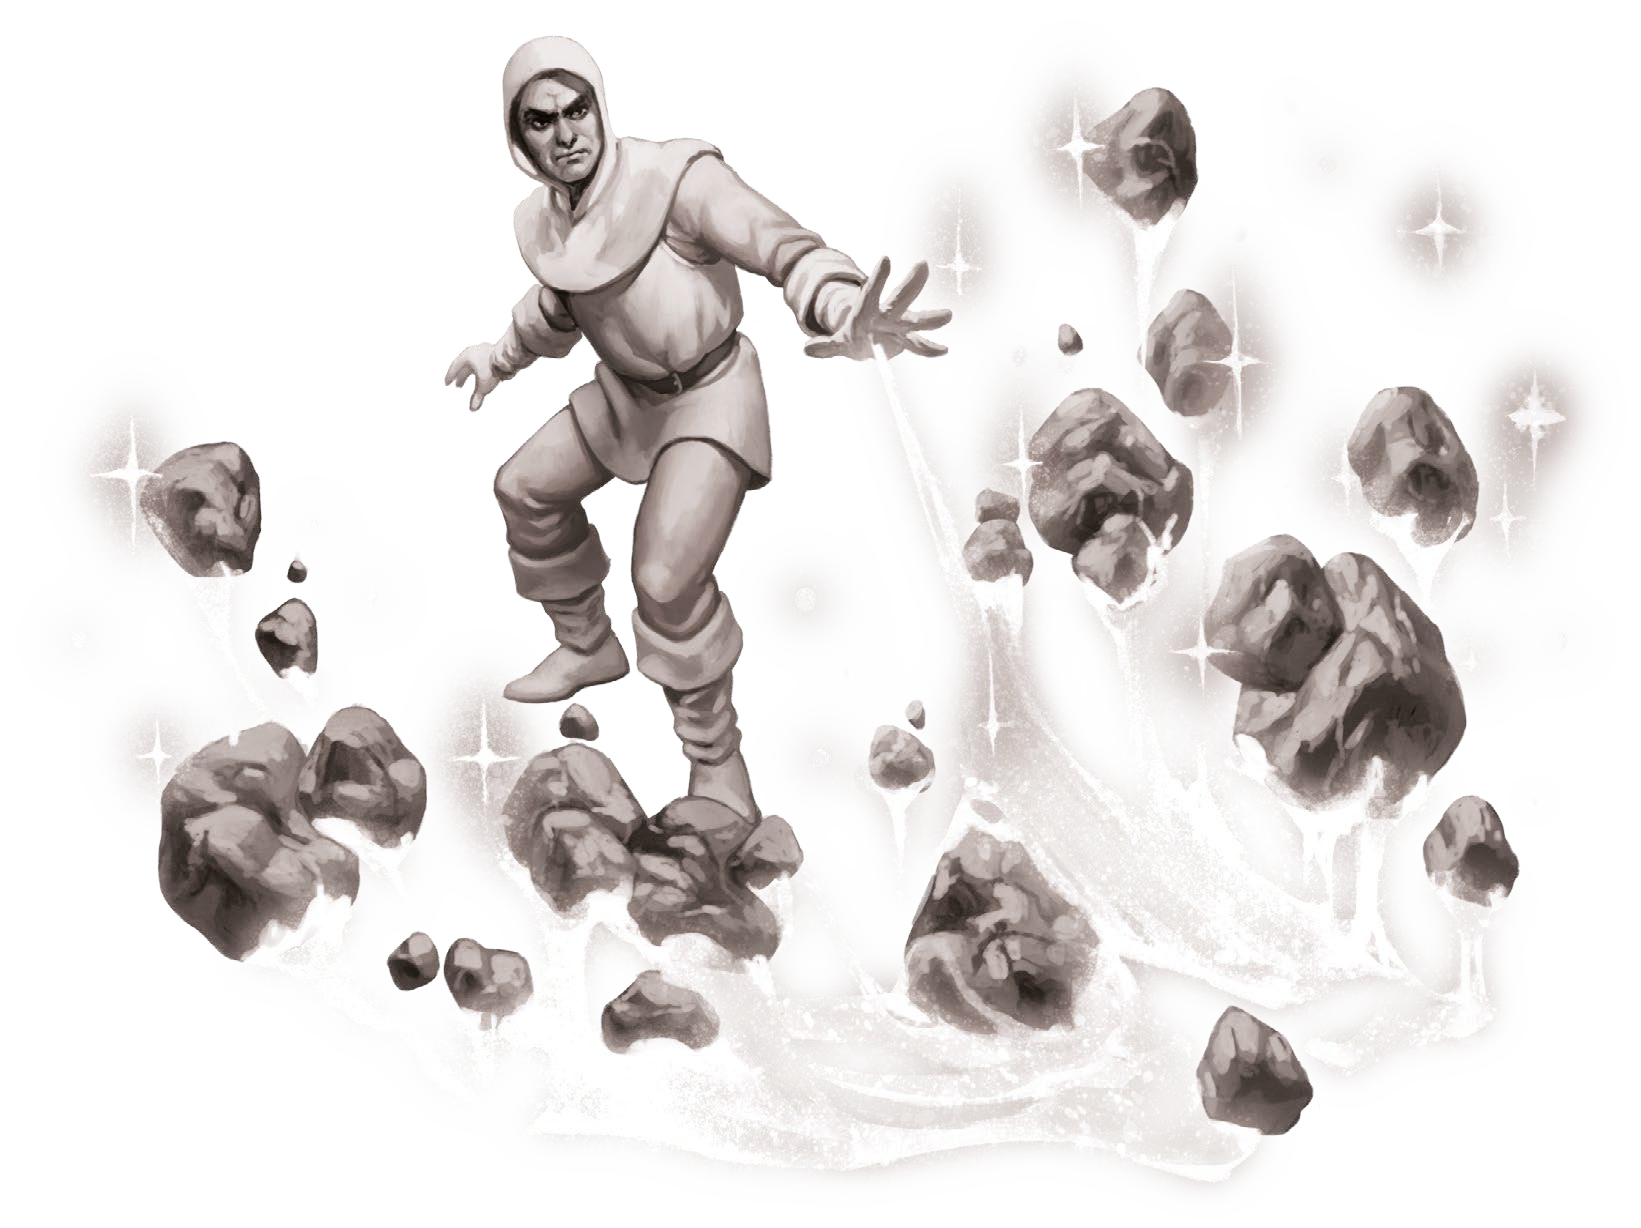
\includegraphics[width=0.5\linewidth]{\art/land_mine.png}
\end{center}

\subsection*{War Machines}
Added by the Rampart expansion.
War Machines\index{War Machines} are permanent Cards that can be bought at either a Trading Post or a War Machine Factory.
If you buy one at the Trading Post, \textbf{you cannot use} any of the other normal functions of that Field during that Visit.
War machines are also more expensive at the Trading Post.\par
\medskip
\begin{minipage}[h]{\linewidth}
  \begin{center}
    \textbf{War Machine Factory}\medskip
  \end{center}
  \framedimage[\linewidth]{\map_locations/war_machine_factory.jpg}
  \footnotesize{Category: \textbf{Revisitable}\\This location allows a Hero to buy a War Machine.}
\end{minipage}

\bigskip

\begin{minipage}[h]{\linewidth}
  \vspace{0pt}
  \centering
  \begin{scriptsize}
    \begin{tikzpicture}
      \draw (0, 0) node[inner sep=0] {\makebox[\textwidth][c]{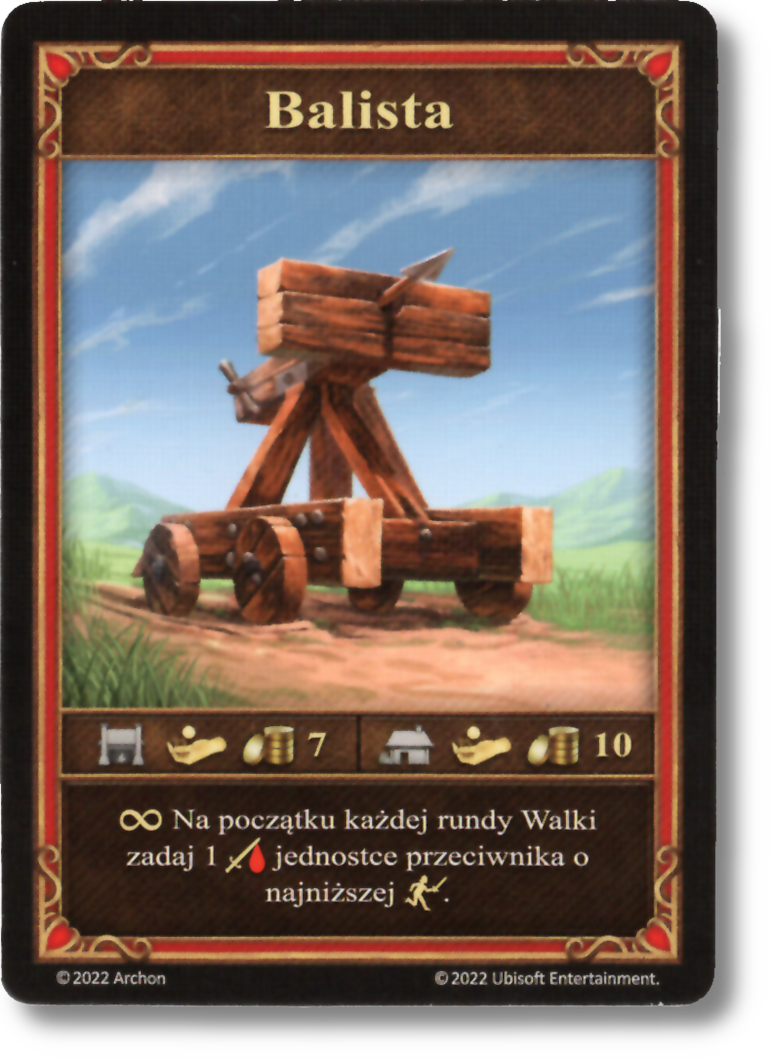
\includegraphics[width=0.8\textwidth]{\cards/war_machine.png}}};
      \draw (0.8, 3.6) node {\encircle{\phantom{.}1\phantom{.}}};
      \draw (0, -2.8) node {\encircle{\phantom{.}2\phantom{.}}};
      \draw (-1.2, -1.7) node {\encircle{\phantom{.}3\phantom{.}}};
      \draw (0.9, -1.7) node {\encircle{\phantom{.}4\phantom{.}}};
    \end{tikzpicture}
  \end{scriptsize}
  \break
  \footnotesize{\textbf{\textit{\textcolor{darkcandyapplered}{War Machine Card}}}}
  \scriptsize
  \begin{multicols}{2}
    \begin{itemize}
      \item[\textbf{1.}] \textbf{Name}
      \item[\textbf{2.}] \textbf{Effect}
      \item[\textbf{\phantom{.}}] \phantom{.}
      \item[\textbf{3.}] \textbf{War Machine Factory cost}
      \item[\textbf{4.}] \textbf{Trading Post cost}
    \end{itemize}
  \end{multicols}
\end{minipage}

\subsection*{Permanent cards}
Added by the stretch goals and Rampart expansions, explained \hyperlink{Playerdecks}{here}.

\subsection*{Events}
Added by the Fortress expansion.
Event cards\index{Event Cards} may be used in games with more than one player.
Shuffle the Event Deck during setup.
At the start of each Resource Round (except the first Round), draw and read the next Event Card after receiving Resources.
The first Event is drawn by the starting player.
\textbf{Change the player who draws the Event in a clockwise order} every time a new Event is drawn.
Resolve any effects in clockwise order starting with the player who drew the Card.
Any cards which were revealed as a part of resolving an Event should be shuffled back into their respective Decks afterwards.

\medskip

\begin{minipage}[h]{\linewidth}
  \vspace{0pt}
  \centering
  \begin{scriptsize}
    \begin{tikzpicture}
      \draw (0, 0) node[inner sep=0] {\makebox[\linewidth][c]{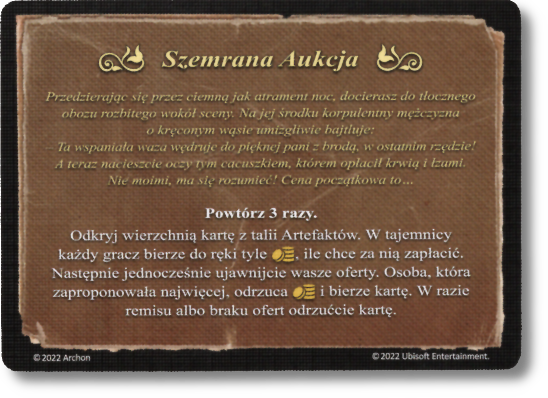
\includegraphics[width=\linewidth]{\cards/event.png}}};
      \draw (1, 1.8) node {\encircle{\phantom{.}1\phantom{.}}};
      \draw (-2, 0.4) node {\encircle{\phantom{.}2\phantom{.}}};
      \draw (2.5, -1.1) node {\encircle{\phantom{.}3\phantom{.}}};
    \end{tikzpicture}
  \end{scriptsize}
  \footnotesize{\textbf{\textit{\textcolor{darkcandyapplered}{Event Card}}}}
  \scriptsize
  \begin{multicols}{2}
    \begin{itemize}
      \item[\textbf{1.}] \textbf{Name}
      \item[\textbf{2.}] \textbf{Fluff}
      \item[\textbf{3.}] \textbf{Effect}
      \item[\textbf{\phantom{.}}] \phantom{.}
    \end{itemize}
  \end{multicols}
\end{minipage}

\subsection*{Summoning}
Some cards from the Inferno expansion may Summon Units\index{Summoning} during Combat.
Place the summoned Unit adjacent to the summoning Unit.
Summoned Units Activate in the Round they were summoned if their Initiative is lower or equal to the Initiative of the currently Activated Unit.
Otherwise, treat them as if they already activated this Combat Round.
After Combat, unless stated otherwise, the Summoned Units are added to your Unit Deck.

\subsection*{Empowered Statistic Cards}\index{Empowered Statistic Card}
Added by the Inferno expansion.
These cards are more powerful versions of the normal Statistics cards.
They have only one effect which is identical to the normal Statistic's Expert Effect, but does not require using your \includesvg[height=10px]{\svgs/expert.svg}.

\begin{scriptsize}
  \begin{tikzpicture}
    \draw (-2, 0) node[inner sep=0] {\makebox[0.47\linewidth][c]{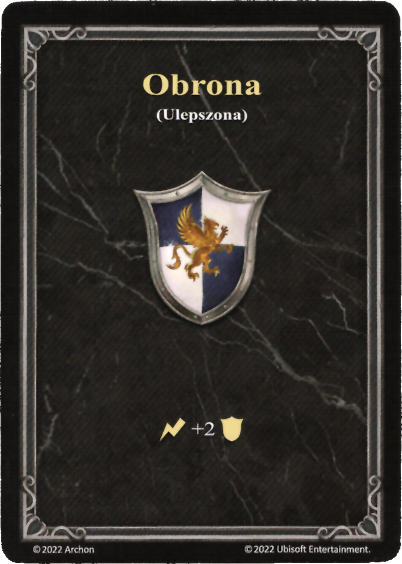
\includegraphics[width=0.47\linewidth]{\cards/empowered_statistic.png}}};
    \draw (2.4, 0) node[inner sep=0] {\makebox[0.47\linewidth][c]{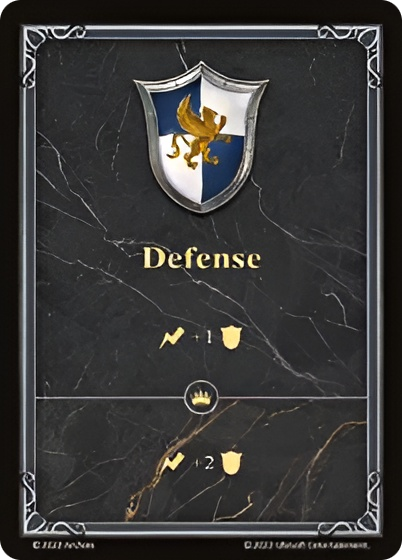
\includegraphics[width=0.47\linewidth]{\cards/statistic.png}}};
    \draw (-1.2, 1.9) node {\encircle{\phantom{.}1\phantom{.}}};
    \draw (3.2, 0.3) node {\encircle{\phantom{.}1\phantom{.}}};
    \draw (-2.7, -1.4) node {\encircle{\phantom{.}2\phantom{.}}};
    \draw (1.7, -0.6) node {\encircle{\phantom{.}2\phantom{.}}};
    \draw (1.7, -1.7) node {\encircle{\phantom{.}3\phantom{.}}};
  \end{tikzpicture}
\end{scriptsize}
\vspace{-2em}
\begin{multicols}{2}
  \centering
  \footnotesize{\textbf{\textit{\textcolor{darkcandyapplered}{Empowered Statistic Card}}}}
  \scriptsize
  \begin{itemize}
    \item[\textbf{1.}] \textbf{Name}
    \item[\textbf{2.}] \textbf{Basic Effect}
  \end{itemize}
  \columnbreak
  \footnotesize{\textbf{\textit{\textcolor{darkcandyapplered}{Statistic Card \phantom{Empowered}}}}}
  \scriptsize
  \begin{itemize}
    \item[\textbf{3.}] \textbf{Expert Effect}
    \item[\textbf{\phantom{.}}] \phantom{.}
  \end{itemize}
\end{multicols}

\subsection*{Random Town}\index{Random Town}
Added by the Inferno expansion.
When this Field is revealed, all players roll 2 \includesvg[height=10px]{\svgs/resource_die.svg}.
The highest roller chooses an unused Faction.
The random Town is defended by Units from that Faction.
They have a "Pack" of \includesvg[height=10px]{\svgs/bronze.svg}, two "Packs" of \includesvg[height=10px]{\svgs/silver.svg}, and two "Fews" of \includesvg[height=10px]{\svgs/golden.svg} Units.
The \includesvg[height=10px]{\svgs/bronze.svg} Unit is chosen by the player who controls the Units during that Combat.
Flagging it increases \includesvg[height=10px]{\svgs/gold.svg} production by 10, which is also gained immediately if you are the first to Flag it.

\bigskip

\begin{minipage}[h]{\linewidth}
  \begin{center}
    \textbf{Random Town}\medskip
  \end{center}
  \framedimage[\linewidth]{\map_locations/random_town.jpg}
  \small{Category: \textbf{Flaggable}}
\end{minipage}

\end{multicols*}
